\documentclass{ohm_project_description}
\usepackage[english]{babel}

\projecttitle{Markerless Indoor Localization of a Drone without GNSS}
\projectauthor{Mobile Robotics Lab}
\projectdate{2026}

\begin{document}

\maketitle
\thispagestyle{fancy}

\vspace*{-2.5cm}
\begin{figure}[h!]
    \centering
    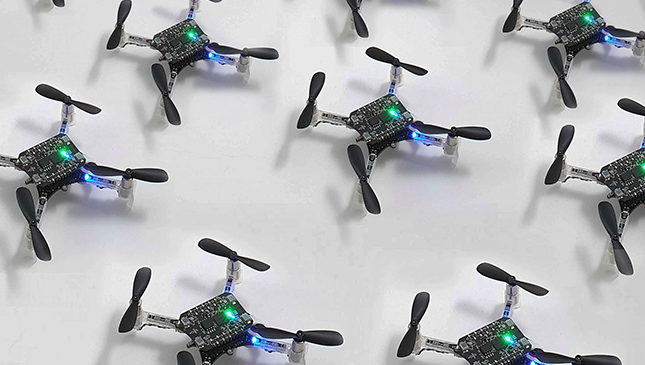
\includegraphics[height=4cm]{img/crazyflies.png}
\end{figure}

The drone used at the AerodrOHM currently determines its position via an external, marker-based tracking system. While this provides very accurate poses, it requires a permanently installed, instrumented flight space and is not available outside of it. The goal of this thesis is to enable the existing drone to localize itself indoors without GNSS and without markers, using only its onboard sensors.

The work builds directly on the existing drone and the established ROS-based system architecture. Suitable onboard sensors (camera, IMU, optionally an optical-flow or depth sensor) are integrated, and a markerless localization method is implemented, for example visual-inertial odometry (VIO) or a visual-SLAM approach. The existing marker-based tracking system at the AerodrOHM serves as ground truth for the evaluation.

\section*{Work Packages}
\begin{itemize}[leftmargin=0.5cm]
    \setlength\itemsep{.1em}
    \item Familiarization with the existing drone platform and the marker-based tracking system at the AerodrOHM
    \item Selection and integration of suitable onboard sensors (camera, IMU, optionally optical-flow or depth sensor)
    \item Implementation of a markerless, GNSS-free localization method (e.g. visual-inertial odometry or visual SLAM)
    \item Integration into the existing ROS system architecture and flight control
    \item Evaluation of accuracy and robustness against the marker-based tracking as ground truth
    \item Flight experiments and documentation of the results at the AerodrOHM
\end{itemize}

\section*{Requirements}
\begin{itemize}[leftmargin=0.5cm]
    \setlength\itemsep{.1em}
    \item Programming skills (Python and/or C++)
    \item Ideally some experience with ROS / ROS 2
    \item Basic knowledge of computer vision and/or state estimation (e.g. Kalman filter)
    \item Interest in drones, sensor integration and localization
    \item Independent and diligent way of working
\end{itemize}

\vspace{0.5cm}
This topic can be completed as a \textbf{project or bachelor's thesis} subject to agreement.

\vfill
\textcolor{ohm_red}{\rule{\linewidth}{0.4mm}}
\textbf{\textcolor{ohm_red}{Mobile Robotics Lab}} \\
\begin{tabular}{@{}ll}
\textbf{Supervisor:} & Prof. Dr. Christian Pfitzner \\
\textbf{E-Mail:}     & \href{mailto:christian.pfitzner@th-nuernberg.de}{christian.pfitzner@th-nuernberg.de} \\
\end{tabular}

\end{document}
